%\newcommand{\argmax}{\operatornamewithlimits{arg\,max}}
%\newcommand{\argmin}{\operatornamewithlimits{arg\,min}}
%\newcommand{\bm}[1]{\boldsymbol{#1}}
%\newcommand{\dataset}{{\cal D}}
%\newcommand{\fracpartial}[2]{\frac{\partial #1}{\partial  #2}}

\def\k{{\mathcal K}}
\def\h{{\mathcal H}}
\def\d{{\bf d}}
\def\K{{\bf K}}
\def\M{{\bf M}}
\def\I{{\bf I}}
\def\U{{\bf U}}
\def\u{{\bf u}}
\def\v{{\bf v}}
\def\a{{\alpha}}
\def\ba{{\bm\alpha}}
\def\eu{{\widehat{\u}_n}}
\def\X{{\mathbf X}}
\def\D{{\mathbf D}}
\def\conv{{\mbox{conv}}}
\def\pd{{\succ\0}}
\def\rk{{\mbox{r}}}
\def\r{{\mathbb R}}
\def\e{{\mathbb E}}
\def\p{{\mathbb P}}
\def\n{{\mathbb N}}

\chapter{Unsupervised Multiple Kernel Learning}


Traditional multiple kernel learning (MKL) algorithms are essentially supervised in the sense that the kernel learning task requires class labels of the training data. However, class labels may not always be available prior to the kernel learning task in some real world scenarios, e.g., some early preprocessing step of a classification task or an unsupervisd learning task such as dimension reduction or clustering. In this chapter, we address a new problem of unsupervised multiple kernel learning (UMKL), which does not require class labels of training data as used in a conventional multiple kernel learning task. As a kernel essentially defines pairwise similarity between any two examples, our unsupervised kernel learning method mainly follows two intuitive principles: (1) a good kernel should allow every example to be well reconstructed from its localized bases weighted by the kernel values; (2) a good kernel should induce kernel values that are coincided with the local geometry of the data. We propose an efficient iterative algorithm to solve the optimization task of the unsupervised multiple kernel learning. Empirical results on a number of UCI data sets verifies the efficacy of our UMKL algorithm.

\section{Introduction of UMKL}

Despite being studied extensively, existing MKL methods are essentially supervised learning which requires class labels of training data available for the learning task. However, the class labels of training data may not always be available for some learning tasks. Examples include unsupervised learning tasks such as dimension reduction, clustering, or some early preprocessing step of a supervised classification task for choosing a kernel before the labeled data arrive. By the above motivations, in this chapter, we address a new problem of {\em Unsupervised Multiple Kernel Learning} (UMKL), which aims to determine a linear combination of multiple kernels by learning only from unlabeled data.

The UMKL task is more challenging than traditional MKL tasks since no class labels are available to guide the learning task. We propose to attack the unsupervised multiple kernel learning problem by exploiting two intuitions: (1) a good kernel should allow every example to be well reconstructed from its localized bases weighted by the kernel values; (2) a good kernel should induce kernel values that are coincided with the local geometry of the data. We formulate the problem as an optimization task by combining the above two intuitions and propose an iterative algorithm to efficiently solve the optimization task.

The rest of this chapter is organized as follows. Section \ref{sec:acml-umkl} presents the problem formulation and the proposed UMKL algorithm. Section \ref{sec:acml-exp} includes our empirical evaluation of the proposed UMKL algorithm.Section \ref{sec:acml-con} concludes this work.


%=======================================================
\section{Framework of UMKL} \label{sec:acml-umkl}
%=======================================================

In this section, we formulate the problem of unsupervised multiple kernel learning and then present an iterative algorithm to solve the optimization task.

%=================================
\subsection{Problem Formulation}
%=================================

Consider a collection of $n$ training samples $\mathcal D = \{(\x_1, y_1),\ldots,(\x_n, y_n)\}$, where $\x_i\in\mathbb{R}^d$ is the input feature vector
and $y_i$ is the unknown class label of $\x_i$, and a set of $m$ predefined kernel functions $\{k_t(\cdot,\cdot),t=1,\ldots,m\}$. The goal of an Unsupervised Multiple Kernel Learning (UMKL) task is to find an optimal linear combination of the $m$ kernel functions, i.e., $k^*(\cdot,\cdot)\in\k_{conv}$, where $\k_{conv}$ is defined as follows:
\begin{equation}
\k_{conv} \!=\!\Big\{k(\cdot,\cdot) \!=\! \sum_{t=1}^m \mu_t k_t(\cdot,\cdot): \sum_{t=1}^m\mu_t  \!=\! 1,\mu_t \!\geq\! 0\Big\}\label{eqn:convex-mkl}
\end{equation}
Unlike supervised MKL, the key challenge of UMKL is how to seek the optimal kernel $k^*(\cdot,\cdot)$ purely from the unlabeled training data. In other words, we need some principles/intuitions to guide the kernel learning task, which should be independent of class labels.

\if 0 We deem kernel as the prior knowledge of the similarity among data, which should be independent of labels. The motivation here is inspired by \cite{nips/YuZG09}, which consists of two pars:\fi

To attack the challenge, we propose to formulate the unsupervised multiple kernel learning task by exploiting the following two intuitive principles:
\begin{itemize}
\item A good kernel should enable each training instance to be well reconstructed from the localized bases weighted by the kernel values. In other words, for each $\x_i$ we expect the optimal kernel can minimize the approximation error $\|x_i-\sum_jk_{ij}\x_j\|^2$;
\item A good kernel should induce kernel values that are coincided with the local geometry of the training data. This is equivalent to finding the optimal kernel that minimizes the distortion over all training data $\sum_{ij}k_{ij}\|\x_i-\x_j|^2$.
\end{itemize}

Besides, we also exploit the locality preserving principle, which has been shown effective for many unsupervised dimension reduction and semi-supervised learning tasks.In particular, to infer such a local structure, we introduce a set of local bases for each $\x_i\in\mathcal X$, denoted $\mathcal B_i\subset\mathcal X$, which is used to reconstruct sample $\x_i$ and compute the distortion as well. Combining the above principles, we have the final optimization for UMKL:
\begin{eqnarray}
\min_{k, \mathcal B} \frac{1}{2}\sum_{i=1}^n \bigg\| \x_i - \sum_{\x_j\in\mathcal B_i} k_{ij}\x_j \bigg\|^2 + \gamma_1\sum_{i=1}^n\sum_{\x_j\in\mathcal B_i} k_{ij}\big\| \x_i - \x_j \big\|^2 + \gamma_2\sum_i| \mathcal B_i |
\end{eqnarray}
where both the target kernel $k\in \k_{conv}$ and the local basis set $\mathcal B_i$ are unknown variables to be optimized, $\gamma_1$ controls the trade-off between the coding error and the locality distortion, $\gamma_2$ controls the size of local basis set.

To simplify the formulation, for each $\x_i$, we introduce a vector $\d \in\{0,1\}^n$ to indicate its neighbors, i.e., $\mathcal B_i =\{\x_j: d_j\neq0\}$. As a result, the optimization problem can be re-written in a matrix-based form:
\begin{eqnarray}
\hspace{0cm}&\min_{\bm\mu,\D}& \!\!\!\!\frac{1}{2} \Big\| \X \big(\I \!-\! \K\!\circ\!\D\big) \Big\|^2_F \!+\! \gamma_1\tr\K\!\circ\!\D\!\circ\!\M\big(\1\1^\top\big) + \gamma_2 \| \D \|_{1,1} \label{eqn:obj}\\
\hspace{0cm}&\st& [\K]_{ij}=\sum_{t=1}^m\mu_tk^t(\x_i, \x_j), 1\leq i, j \leq n, \bm\mu^\top\1 = 1, \bm\mu\geq 0, \D\in\{0,1\}^{n\times n} \nonumber,
%\nonumber,\\\hspace{0cm}&&
\end{eqnarray}
where the $i$-th column of $\X$ is the point $\x_i$, matrix $[\M]_{ij} := \x_i^\top\x_i+\x_j^\top\x_j - 2\x_i^\top\x_j$ is the Euclidean distance matrix defined on $\X$, $B\in\n_+$ is the parameter controls the size of $\mathcal B_i$ for each $\x_i$. For the above notations, $\circ$ denotes an element-wise multiplication of two matrices, $\|\cdot\|^2_F$ denotes the Frobenius-norm of a matrix, and $tr$ denotes the trace of a matrix.

The presented formulation essentially treats the kernel evaluation $\bm\kappa_i$ as a local coding coordinate of $\x_i$. With the additional constraint $\bm\kappa^\top\1 = 1$, such a local coding system allows a linear approximation of an target function, guaranteed by\cite{nips/YuZG09}:
\begin{theorem}
Let $(\bm\kappa, \mathcal B)$ be an arbitrary coordinate coding on $\mathbb R^d$. Let $f$ be an $(\alpha, \beta, p)$-Lipschitz smooth function, i.e., $| f(\x) - f(\x')| \leq \alpha \| \x - \x'\|$ and $|f(\x') - f(\x) - \nabla f(\x)^\top(\x' - \x)| \leq \beta\|\x - \x'\|^{1+p}$, $\alpha, \beta>0, p\in(0, 1]$. We have for all $\x\in\mathbb R^d$:
\[
\Big| f(\x) - \sum_{\x_j\in\mathcal B}\kappa(\x_i, \x_j)f(\x_j) \Big| \leq \alpha\| \x - \sum_j\kappa_j\x_j \| + \beta \sum_{\x_j\in\mathcal B}| \kappa(\x_i, \x_j) | \| \x_i - \x_i \|^{1+p}.
\]
\end{theorem}
For practical purpose, we remove the constraint $\bm\kappa^\top\1=1$. Instead, we deem the coding as kernel evaluation result, which is sampled from a predefined set $\mathcal K_{conv}$. Moreover, for each data point $\x_i$, we learn a set of local bases, rather than a global basis set. This allows further locality characterization of the data. Such local bases are also useful for discovering the data topology, which is essential for data embedding tasks.

%=================================
\subsection{Iterative Optimization Algorithm}
%=================================

It is not difficult to see that the optimization task (\ref{eqn:obj}) is essentially a mixed integer programming, which is not easy to solve directly. In our approach, we propose an iterative optimization algorithm by alternatively solving $\bm\mu$ and $\D$, which is in spirit to \cite{icml/TanWT10}.

%++++++++++++++++++++++
\subsubsection{Solving $\bm\mu$ by Fixing $\D$}
%++++++++++++++++++++++

We first solve $\bm\mu$ by assuming the values of $\D$ have been identified. The objective reduces to
\begin{eqnarray}
J(\bm\mu) = \bm\mu^\top\bigg(  \sum_{t=1}^m \sum_{i=1}^n\bm\kappa_{t,i}\bm\kappa_{t,i}^\top\circ\mathbf d_i\mathbf d_i^\top\circ\mathbf P              \bigg)\top\bm\mu + \mathbf u^\top\bm\mu,
\end{eqnarray}
where $[\mathbf u]_t:= \sum_{i=1}^n(\mathbf v\circ\mathbf d_i - 2\mathbf p_i\circ\mathbf d_i)^\top\bm\kappa_{t,i}$, $\mathbf P = \X^\top\X$ is a linear kernel, $\bm\kappa_{t,i} :=[k^t(\x_i,\x_1),\ldots,k^t(\x_i,\x_n)]^\top$ is the $i$-th column of the $t$-th kernel matrix,  $\mathbf p$ and $\mathbf v$ are the columns of $\mathbf P$ and $\M$ corresponding to $\x_i$, separately.

As a result, the original optimization problem (\ref{eqn:obj}) w.r.t. $\bm\mu$ is re-formulated into a quadratic program~\cite{Boyd} which can be solved efficiently with an off-the-shelf optimization toolkit.

%++++++++++++++++++++++
\subsubsection{Solving $\D$ by Fixing the Kernel} % Greedily}
%++++++++++++++++++++++

The $i$-th column $\mathbf d_i$ of $\D$ is a binary vector indicating the set of localized bases of sample $\x_i$. Note that the columns of $\D$ are independent of each others, i.e., the solution $\mathbf d_i$ of a specific sample $\x_i$ would not affect the bases of other samples. Therefore, we can solve each column $\mathbf d_i$ of $\D$ separately.

At the beginning, we need to find the local basis set for each training sample. To this end, we adopt sparse coding to initialize $\D$, which is formulated into:
\begin{equation}
J(\mathbf d) = \frac{1}{2}\Big\| \x_i - \sum_{j\neq i}d_j\x_j \Big\|^2_2 + \gamma_2\| \mathbf d \|_1. \label{eqn:sparse-coding}
\end{equation}
Note here we relax the binary indicating vector $\mathbf d$ to continuously valued vector. This is a typical sparse coding problem, which can be solved efficiently by feature-sign algorithm \cite{nips/Lee06}.

Assume the we have learned a kernel with the feature mapping function $\Phi$, i.e., $k_{ij} = \Phi(\x_i)^\top\Phi(\x_j)$. The sparse coding (\ref{eqn:sparse-coding}) can be kernelized as
\begin{eqnarray}
J(\mathbf d) &=& \frac{1}{2}\| \Phi(\x_i) - \sum_{j\neq i}d_j\Phi(\x_j) \|_2^2+\gamma_2\| \mathbf d \|_1 \nonumber\\
&=& \frac{1}{2}\big(k_{ii} + \mathbf d_i^\top\mathbf K\mathbf d_i - 2\mathbf d_i^\top\bm\kappa\big) + \gamma_2\| \mathbf d_i \|_1 \nonumber,
\end{eqnarray}
where $\bm\kappa=[k(\x_i,\x_j)]_j$ abbreviates the $i$-th column of the kernel matrix $\mathbf K$. Besides the relaxation of $\D$, another scheme is to propose some greedy algorithm to tackle the original mixed integer programming problem. To this end, we formulate (\ref{eqn:obj}) w.r.t. $\mathbf d$ by
\begin{equation}
J(\mathbf d) = \mathbf d^\top\big(\bm\kappa\bm\kappa^\top\circ\mathbf P\big)\mathbf d + \big(\bm\kappa\circ\mathbf v- 2\bm\kappa\circ\mathbf p\big)^\top\mathbf d, \label{eqn:d}
\end{equation}
where the common subscript of $\mathbf d, \bm\kappa, \mathbf p, \mathbf v$ are omitted.

Let $\U$ abbreviate $\bm\kappa\bm\kappa^\top\circ\mathbf P$, and $\v$ abbreviate $\bm\kappa\circ\mathbf v- 2\bm\kappa\circ\mathbf p$. We solve $\mathbf d$ by a greedy algorithm. Initially, we set all the entries of $\mathbf d$ to zero. At each greedy step, we add one sample into the basis set of $\x$, which implies to set one component of $\mathbf d$ to 1. We choose the component as the one which minimizes the increase of $J(\mathbf d)$. This process is iterated until $B$ entries of $\mathbf d$ have been set to 1.

Assuming each dimension of $\x$ is nonnegative, one can show immediately that $J(\mathbf d)$ is a sub-modular function, i.e., $J(\mathbf d^1) + J(\mathbf d^2) \geq J(\mathbf d^1 | \mathbf d^2) + J(\mathbf d^1 \& \mathbf d^2)$, where $|$ and $\&$ are the bit-wise ``or" and ``and" operation. The following theorem guarantees the performance of greedy selection of $\mathbf d$:
\begin{theorem}
Let $\mathbf d^*$ denote the optimal solution of (\ref{eqn:d}), and $\hat{\mathbf d}$ denote the approximation solution found by the greedy algorithm. We have
\[
J(\hat{\mathbf d}) \geq J(\mathbf d^*)(1 - 1/ e),
\]
if $J(\mathbf d)$ satisfies the following conditions: 1) $J(\mathbf d^1)\leq J(\mathbf d^2)$ if $\mathbf d^1\subset \mathbf d^2$; 2) $J(\mathbf d)$ is a submodular function, and 3) $J(\mathbf 0)=0$.
\end{theorem}

\begin{algorithm}[!htp]\label{alg:umkl}
\caption{UMKL: Unsupervised Multiple Kernel Learning}
\textbf{Input:} Unlabeled data $\X$, base kernels $\mathcal K_{base} = \{k_1,\ldots,k_m\}$, $\gamma$, $B$; \\
\textbf{Output:} Kernel weight $\bm\mu$, bases indicator matrix $\D$.\\\vspace{-0.1in}
\begin{algorithmic}
[1]\STATE Initialize $[\M]_{ij} = \x_i^\top\x_i + \x_j^\top\x_j - 2\x_i^\top\x_j$, $\bm\mu=\1/m$, $\mathbf P=\X^\top\X$;

\REPEAT

\STATE $\mathbf W = \sum_{t=1}^m \sum_{i=1}^n\bm\kappa_{t,i}\bm\kappa_{t,i}^\top\circ\mathbf d_i\mathbf d_i^\top\circ\mathbf P$;

\STATE $\bm\mu = \argmin_{\bm\mu}\bm\mu^\top\mathbf W\bm\mu + \mathbf u^\top\bm\mu$;

%\STATE $\nabla J =\sum_{i=1}^n\sum_{\x_j\in\mathcal B_i} \Big(k_{ij}\x_j^\top\x_j - \x_i^\top\x_j + \gamma\|\x_i - \x_j\|^2\Big)k_{ij}^t$;

%\STATE $\bm\mu = \bm\mu + \eta\nabla(J)$;

\FOR{each $\x_i$}

\STATE $\U = \bm\kappa\bm\kappa^\top\circ\mathbf P$,$\v = \bm\kappa(\mathbf v - 2\mathbf p)$;

\STATE Set $\mathcal B_i = \emptyset$;

\FOR{$|\mathcal B_i|<B$}

\STATE $\x^* \!=\! \argmin_{\x_j\in\mathcal X\!-\!\mathcal B_i}2\sum_{t:\x_t\in\mathcal B_i}U_{tj}\!+\!U_{jj} \!+\! v_j$;

\STATE $\mathcal B_i=\mathcal B_i\cup\{\x^*\}$;

\ENDFOR

\ENDFOR

\UNTIL{convergence}

\end{algorithmic}
\end{algorithm}

After kernel learning, the kernel can be used in classification, or other semi-supervised and unsupervised tasks, such as dimension reduction, etc.

%=======================================================
\section{Experiments}\label{sec:acml-exp}
%=======================================================
In order to examine the efficacy of the proposed UMKL algorithm, we apply the proposed UMKL algorithm in two scenarios: (i) a pre-processing tool to find an appropriate kernel for classification task, and (ii) a nonlinear dimension reduction tool for machine learning and data mining tasks.

%=================================
\subsection{Experimental Testbed and Setup}
%=================================

We evaluate the performance of the proposed UMKL algorithms for binary classification tasks over a testbed of publicly available data sets as shown in Table 1\footnote{http://www.csie.ntu.edu.tw/~cjlin/libsvmtools/datasets/}
\footnote{http://www.fml.tuebingen.mpg.de/Members/raetsch/benchmark}.

\begin{table*}[!thbp] \label{table:dataset}
%\vspace{-0.2in}
\centering\caption{The statistics of the 12 binary-class data sets used in our experiments.}
%\vspace{-0.1in}
\begin{center}
%\begin{footnotesize}
%\scriptsize
\begin{tabular}{l|rrrrrrrrrr}
\hline
Data Set    &Breast  &Diabetes   &Waveform  &Sonar &Liver  &German\\%&Adult&Ionosphere
\hline
\hline
\# instances      &683  &768    &400    &208    &345    &1,000 \\%&1,605&351
\# dimensions &10   &8  &21 &60 &6  &24\\%&123&33
\hline
\hline
Data Set    &Australian  &Thyroid &Heart    &Banana   &Titanic  &FlareSolar\\%&Splice&Ringnorm
\hline
\hline
\# instances      &690    &140    &270    &400    &150    &666   \\%&1,000&400
\# dimensions  &14 &5  &13 &2  &3  &9    \\% &60&20
\hline
\end{tabular}
%\end{footnotesize}
\end{center}
%\vspace{-0.1in}
\end{table*}

Following the settings of previous MKL studies~\cite{nips/XuJKL08}, for each data set, we create the set of base kernels $\k$ as follows: %for MKL as in
(1) Gaussian kernels with 10 different widths ($\{2^{-3},2^{-2},\ldots,2^6\}$) on all features and on each single feature; (2) polynomial kernels of degree 1 to 3 on all features and on each single feature. Each base kernel matrix is normalized to unit trace. The training instances are normalized to be of zero mean and unit variance, and the test instances are also normalized using the same mean and variance of the training data. To get stable results, for each data set, we repeat each algorithm 20 times and compute the average results of the 20 runs.


%=================================
\subsection{Experiment I:Unsupervised MKL versus Supervised MKL}
%=================================

The first experiment is to examine whether the proposed UMKL algorithm can produce good results comparing it with traditional supervised kernel learning (SKL) algorithms on the same set of training data.

Specifically, we have compared the following algorithms:
\begin{itemize}
  \item []\hspace{-1cm}{\bf AvgKernel}: The average combination of multiple kernels;
  \item []\hspace{-1cm}{\bf MKL$^{\mathrm{Level}}$}: The convex multiple kernel learning algorithm, that is, the target
         kernel class is $\k_{conv}$ defined in (\ref{eqn:convex-mkl}). We use the
         extended level method \cite{nips/XuJKL08} to learn the kernel;
  \item []\hspace{-1cm}{\bf LpMKL}: The MKL algorithm with $L_p$ norm regularization over
        the kernel weight \cite{nips/KloftBSLMZ09}. We adopt their cutting plane
        algorithm with second order Taylor approximation of $L_p$;
  \item []\hspace{-1cm}{\bf GMKL}: The Generalized MKL algorithm in \cite{icml/VarmaB09}. The target kernel class is the Hadamard product of single Gaussian kernel defined on each dimension;
  \item[]\hspace{-1cm}{\bf KTA}: The Two-stage Kernel Learning by Kernel Target Alignment algorithm in \cite{icml/Cortes09};
    \item[]\hspace{-1cm}{\bf UMKL}: The proposed Unsupervised MKL method with the greedy base set selection\footnote{We also evaluated another variant of the UMKL algorithm by the sparse coding solution. We found that it is always slightly worse than the greedy algorithm for most cases.};  We first learn the kernel by UMKL and then apply the kernel for learning an SVM classifier.
\end{itemize}

For parameter settings, the regularization parameter $C$ in SVM for all the compared methods is determined by 5-fold cross validation on the training data over the range of $\{10^{-2}, 10^{-1}, \ldots, 10^2\}$. For a fair comparison, the same set of base kernels was adopted by MKL$^{\mathrm{Level}}$, LpMKL, KTA, and UMKL.  For LpMKL, we examine $p=2,3,4$ and report the best result.

For each data set, we randomly sample $50\%$ of all instances as training data, and use the rest as test data. The classification accuracy is shown in Table 2, from which we can draw two observations.


\begin{table*}[!thbp] \label{table:acml-exp1-result}
\vspace{-0.1in} \centering \caption{The evaluation of classification performance by comparing with a number of different algorithms. Each element in the table shows the mean and standard deviation of classification accuracy (\%). The relative ranking of different MKL algorithms on each data is shown in (). The last row shows the average rank score over all data sets achieved by each algorithm. The {\bf bold} element indicates the best performance.}
\begin{center}
%\setlength{\tabcolsep}{4.5pt}
%\setlength{\extrarowheight}{1.5pt}
{%\small
\begin{tabular}{l|l|lllll}
\hline
Data Set  &AvgKernel & MKL$^{\mathrm{level}}$
    &LpMKL  &GMKL  &KTA &UMKL\\
\hline
\hline              %SVM                 LevelMKL            LpMKL               GMKL               IKL                                KDL                     DMKL
Breast          &95.5$\pm$1.0      &96.5$\pm$0.8 &96.2$\pm$0.7  &{\bf 97.0$\pm$1.0}  &96.5$\pm$0.8 &{\bf 97.0$\pm$0.6}\\
Diabetes       &65.4$\pm$2.0  &75.8$\pm$2.5  &72.6$\pm$2.5 &66.4$\pm$2.5   &75.2$\pm$3.3 &{\bf 77.1$\pm$2.3}\\
Titanic         &76.2$\pm$4.2     &77.1$\pm$2.9    &77.0$\pm$3.0 &76.7$\pm$3.1       &78.9$\pm$1.2 &{\bf79.2$\pm$2.5}\\
Heart          &75.6$\pm$6.0    &83.0$\pm$2.9   &76.7$\pm$3.8 &77.0$\pm$3.6    &82.0$\pm$1.9 &{\bf 84.7$\pm$2.6}\\
German          &69.5$\pm$1.5   &71.4$\pm$2.8   &{\bf74.3$\pm$1.4} &70.4$\pm$1.6   &72.1$\pm$1.1 &{\bf74.8$\pm$1.8}\\
Australian     &66.7$\pm$5.6  &85.0$\pm$1.5  &84.5$\pm$1.6 &80.0$\pm$2.3 &{\bf 87.2$\pm$0} &86.3$\pm$1.3\\
Banana         &86.1$\pm$2.3     &90.2$\pm$2.0   &87.5$\pm$2.6 &83.4$\pm$2.7 &{\bf 92.1$\pm$1.7} &90.2$\pm$1.9\\
Thyroid        &82.6$\pm$4.4  &92.9$\pm$2.9    &93.1$\pm$2.2 &94.6$\pm$2.1 &{\bf 97.9$\pm$1.3} &91.2$\pm$2.7\\
FlareSolar     &64.8$\pm$1.6 &{\bf67.6$\pm$2.0}   &64.8$\pm$1.8 &65.3$\pm$1.8  &66.7$\pm$2.3  &{\bf67.8$\pm$1.8}\\
Waveform    &73.5$\pm$7.1 &88.2$\pm$1.6   &{\bf 88.9$\pm$2.0} &88.2$\pm$1.8 &88.5$\pm$2.5 &88.4$\pm$2.5\\
Sonar         &59.1$\pm$9.7 &78.3$\pm$3.5&{\bf 84.8$\pm$3.2} &78.8$\pm$4.6 &81.3$\pm$2.9 &81.0$\pm$2.9\\
Liver       &57.6$\pm$2.3       &62.3$\pm$4.5 &{\bf 69.4$\pm$2.9} &63.6$\pm$2.6 &68.7$\pm$1.5 &68.3$\pm$4.3\\
\hline
\end{tabular}
}
\end{center}
%R\vspace{-0.2in}
\end{table*}


\begin{figure*}[!t]
\begin{center}
\subfigure[heart]{
\includegraphics[width=2.8in]{figures/acml-heart.eps}
}
\subfigure[titanic]{
\includegraphics[width=2.8in]{figures/acml-titanic.eps}
}
\caption{Classification accuracy of UMKL and KTA by varying \#train/\#test. }
\end{center}
\end{figure*}

First, UMKL is comparable with supervised kernel learning algorithms. Among the evaluated 12 data sets, UMKL reports 6 best results, which is the largest among all the evaluated methods. None of the compared 4 algorithms, i.e., MKL, LpMKL, GMKL, and KTA, can outperform the proposed UMKL algorithm significantly. The average rank of UMKL is comparable with KTA. These three algorithms are significantly better than MKL and GMKL. This result verifies the efficacy of UMKL clearly. When the half of the data have labels for training, SKL and UMKL, which does not use the label information, produce similar classification accuracy.

Second, among the SKL algorithms, KTA yield the best performance. The average rank of KTA among SKL algorithms is the best. Traditional MKL cannot result in the best accuracy on any evaluated data sets. The results of KTA on {\em thyroid} are statistically significant better than other SKL methods. Figure 1 illustrates the performance comparison of both UMKL and KTA algorithms by varying the fraction of training data instances on two datasets. For most situtations, the performance of UMKL is consistently better or comparable to that of the KTA algorithm, which again validates the efficacy of the unsupervised multiple kernel learning algorithm.


%=================================
\subsection{Experiment II: UMKL for Dimensionality Reduction}
%=================================

Our second experiment is to examine if the proposed UKML algoithm is effective for an unsupervised dimension reduction task using kernel techniques. To this purpose, we apply the UMKL algorithm as a tool to learn an appropriate kernel function for Kernel PCA, which is a classical nonlinear dimensionality reduction technique that chooses the dominating principle component in the feature space. Typically, it is often non-trivial to select the appropriate kernel based on given data for kernel PCA.

Specifically, in this experiment, we compare the following different approaches of choosing kernels for kernel PCA towards dimension reduction tasks:
\begin{itemize}
\item [] \hspace{-1cm}{\bf Guassian}: We consider a single Guassian kernel, where the band-width parameter $\sigma$ is chosen empirically from the data (we simply fix $\sigma=1$ in our experiments;
\item []\hspace{-1cm}{\bf Average}: The average kernel by combining the set of multiple kernels via a uniformly linear combination approach, where the set of multiple kernels is the same as the previous experiment;
\item []\hspace{-1cm}{\bf C-UKL}: The unsupervised kernel learning learning algorithm aiming to maximize margin of the data (cluster assumption on the data), proposed by \cite{nips/ValizadeganJ06};
\item []\hspace{-1cm}{\bf UMKL}: The proposed UMKL algorithm to identify the appropriate linear combination of multiple kernels on the same set of multiple kernels.
\end{itemize}

\begin{table*}[!thbp] \label{table:KPCA}
%\vspace{-0.1in}
\centering \caption{The classification accuracy of a 5-NN classifier on the projected data by KPCA with three different kinds of kerenls, i.e., a gaussian kernel with fixed sigma=1, the average combination of multiple kernels, and the kernel learned by UMKL on 9 benchmark data sets. The parameter $B$ of UMKL is fixed to 10. The {\bf bold} element indicates the best performance.}
\begin{center}
%\setlength{\tabcolsep}{4.5pt}
%\setlength{\extrarowheight}{1.5pt}
{%\small
\begin{tabular}{l|l|l|l|l|}
\hline
Data Set  & Gaussian Kernel &Average Kernel &C-UKL
    &UMKL$^{\mathrm{Sub}}$\\
\hline
\hline              %SVM                 LevelMKL            LpMKL               GMKL               IKL                                KDL                     DMKL
Breast          &95.1$\pm$0.8      &92.7$\pm$2.7 &94.8$\pm$1.0   &{\bf95.2$\pm$1.3}  \\
Diabetes       &64.6$\pm$2.4  &65.1$\pm$2.3  &64.2$\pm$2.4   &{\bf66.3$\pm$2.5} \\
Heart          &56.2$\pm$3.5    &61.5$\pm$5.8   &55.7$\pm$3.4 &{\bf72.4$\pm$5.9} \\
German          &63.9$\pm$1.7   &64.3$\pm$1.9   &63.4$\pm$1.8   &{\bf64.9$\pm$2.2}\\
Australian     &57.7$\pm$2.3  &55.9$\pm$2.6  &69.4$\pm$2.9   &{\bf72.9$\pm$3.8} \\
FlareSolar     &61.9$\pm$3.4 &62.5$\pm$3.6   &62.8$\pm$3.5   &{\bf63.0$\pm$3.5}\\
Waveform    &59.4$\pm$3.5 &63.2$\pm$4.1   &63.9$\pm$5.8 &{\bf 76.9$\pm$3.9} \\
Sonar         &50.7$\pm$5.0 &56.7$\pm$5.8 &54.6$\pm$6.7 &{\bf 57.0$\pm$7.2} \\
Liver       &52.9$\pm$4.5       &52.0$\pm$3.3 &{\bf 53.4$\pm$3.4}   &{\bf 53.2$\pm$3.3} \\
\hline
\end{tabular}
}
\end{center}
%R\vspace{-0.2in}
\end{table*}


In this experiment, for each of the above approaches, we apply it to reduce data from the original dimensionality to 2 dimensions, and then adopt a 5-nearest neighbor classification scheme to evaluate the classification performance on the reduced data.  For each data set, we randomly sample $50\%$ of all instances as training data, and use the rest as test data. To obtain stable results, for each data set, we repeat the randomized sampling process 20 times, run each algorithm on these randomly sampled training/test data, and finally compute the average results of each algorithm over these 20 runs. We adopt 9 benchmark datasets as used in Experiment I \footnote{Note that we do not use three of the datasets (i.e., Banana, Titanic, and THyroid) because of their original dimensionality is already very slow (e.g., 2,3,5 respectively)}.



\begin{figure*}[!ht]\label{figure:acml-kernel-pca}
\hspace{-0.1in}
\begin{center}
%\subfigure[5-NN classification after KPCA]{
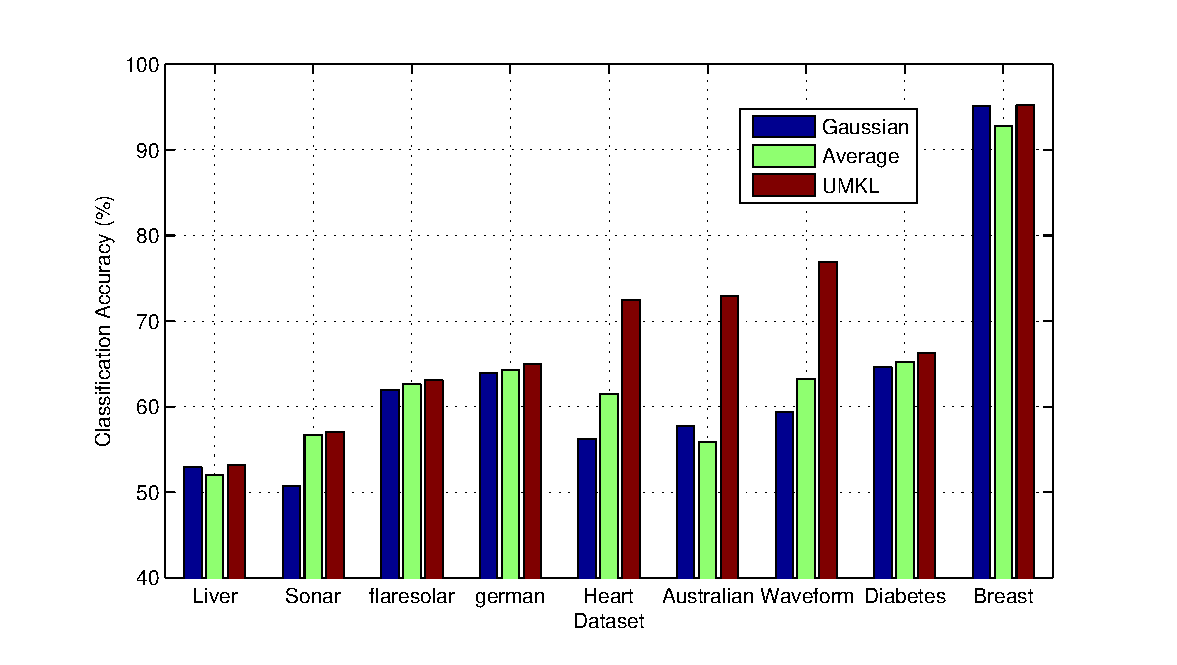
\includegraphics[width= 6.5 in]{figures/acml-KernelPCA.eps}
%}
\caption{The classification accuracy of 5-NN after KPCA with Gaussian kernel with sigma=1,the average combination of multiple kernels, the kernel learned by UMKL on 9 benchmark data sets. The parameter $B$ of UMKL is fixed to 10.}
\end{center}
\end{figure*}


Table \ref{table:KPCA} and Figure \ref{figure:acml-kernel-pca} summarize the experimental results of the kernel PCA by three kinds of different kernels for supervised classification tasks. From the results, we could see that the proposed UMKL algorithm is able to learn a better kernel that is considerably more effective than either a single gaussian kernel or an average kernel via a uniformly linear combination for most cases. The results are particularly impressive on several datasets including heart, australian, waveform, where UMKL significantly surpasses the other two approaches.

In addition to the fixed number of reduced dimensions, we also try to examine how the compared algorithms work when applying KPCA to obtain projected data of a varied numbers of dimensions. Figure \ref{figure:acml-kpca} shows the experimental results of evaluating the classification performance on the data by applying KPCA to obtain low-dimensional data of varied numbers of dimensions. From the results, it is clear that UMKL performs consistently better than both the single gaussian kernel and the average kernel on all the cases of varied numbers of dimensions.

Finally, we also evaluate the classification performance by examining the effects of varied numbers of nearest neighbors, i.e., $k$, used in the $k$-NN classifiers. Figure \ref{figure:acml-k-nn} shows the detailed results of classification evaluation by varying the number of nearest neighbors on the heart dataset. The proposed UMKL algorithm consistently surpasses the other two baselines. Figure \ref{figure:acml-kpca-example} gives most results on the other datasets. It is clear that the proposed UMKL algorithm always achieves the best performance for all the datasets.


\begin{figure*}[!ht]\label{figure:acml-kpca}
\hspace{-0.1in}
\begin{center}
\subfigure[5-NN classification after KPCA with varied number of dimensions]{
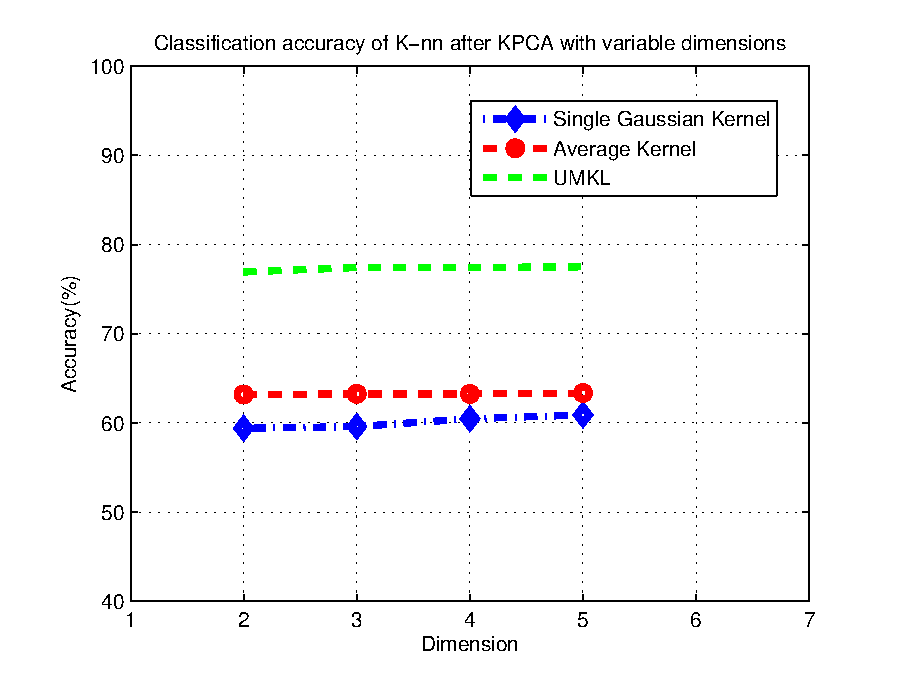
\includegraphics[width= 5 in]{figures/acml-KPCA.eps}
}
\caption{The classification accuracy of 5-NN after KPCA with Gaussian kernel with sigma=1,the average combination of multiple kernels, the kernel learned by UMKL with varied dimensions, on the waveform dataset.}
\end{center}
\end{figure*}

\begin{figure*}[!ht]\label{figure:acml-k-nn}
\hspace{-0.1in}
\begin{center}
\subfigure[K-NN classification after KPCA with varied number of nearest neighbours]{
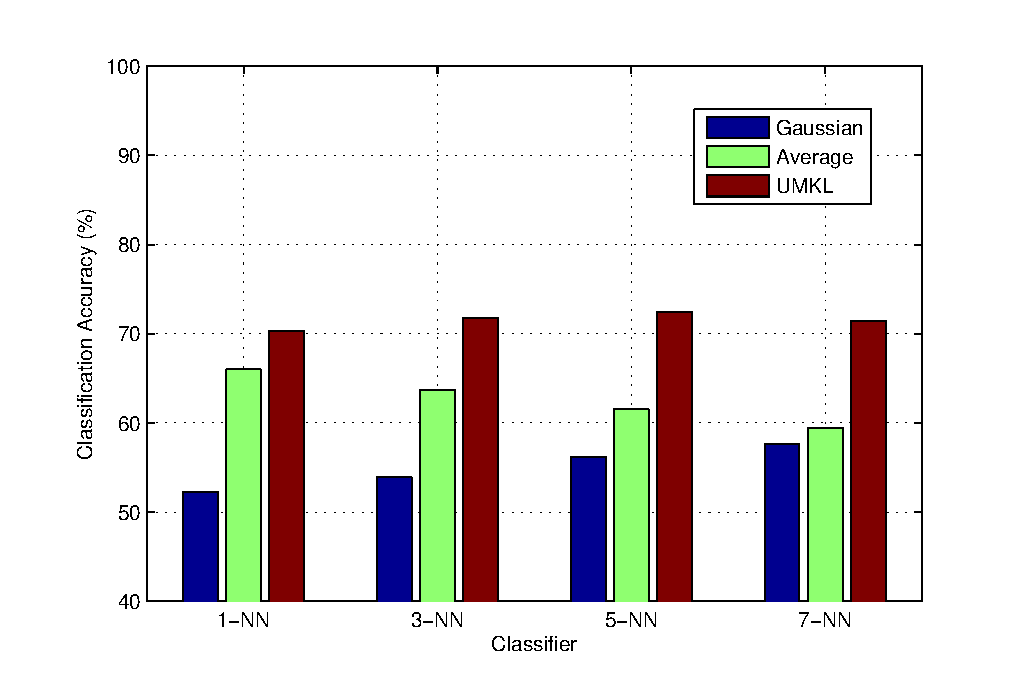
\includegraphics[width= 5 in]{figures/acml-K-NN.eps}
}
\caption{The classification accuracy of k-NN after KPCA with a gaussian kernel with sigma=1, the average combination of multiple kernels, the kernel learned by UMKL with varied number of nearest neighbours, on the heart dataset.}
\end{center}
\end{figure*}

\begin{figure*}[!ht]\label{figure:acml-kpca-example}
\hspace{-0.1in}
\begin{center}
\subfigure[Waveform]{
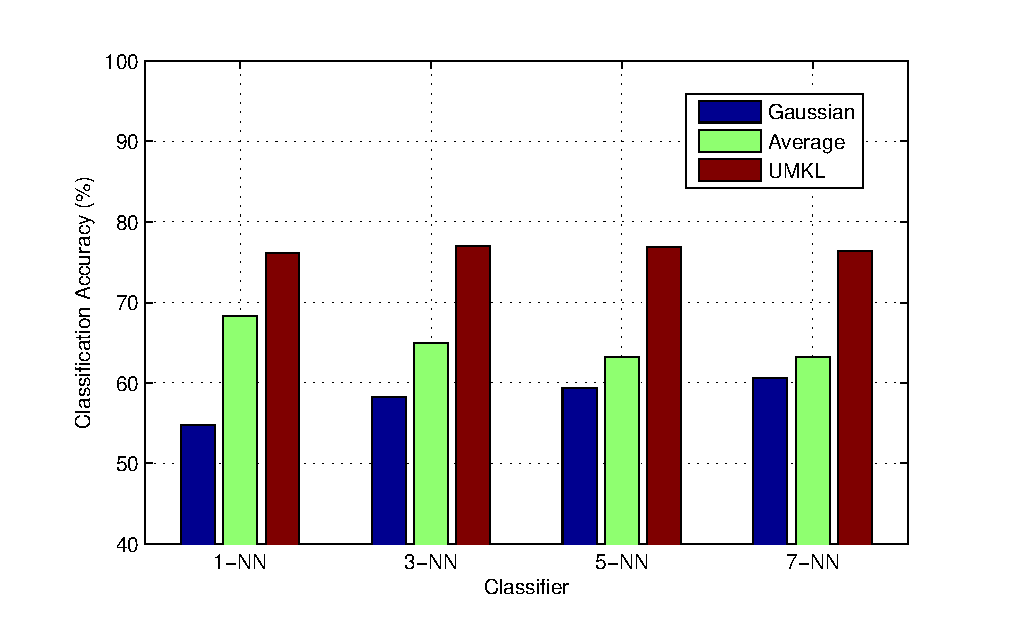
\includegraphics[width=2.5in]{figures/acml-KPCAonwaveform.eps}%1.51
}
\subfigure[Australian]{
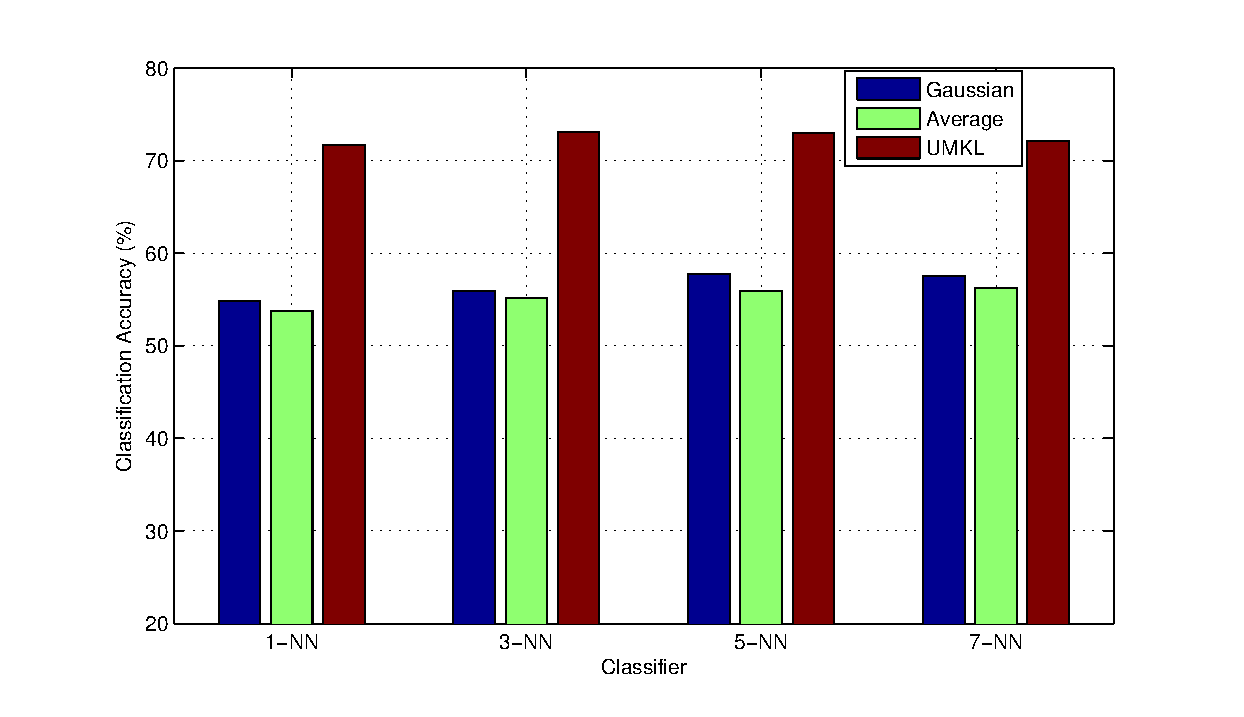
\includegraphics[width=2.5in]{figures/acml-KPCAaustralian.eps}
}
\subfigure[Breast]{
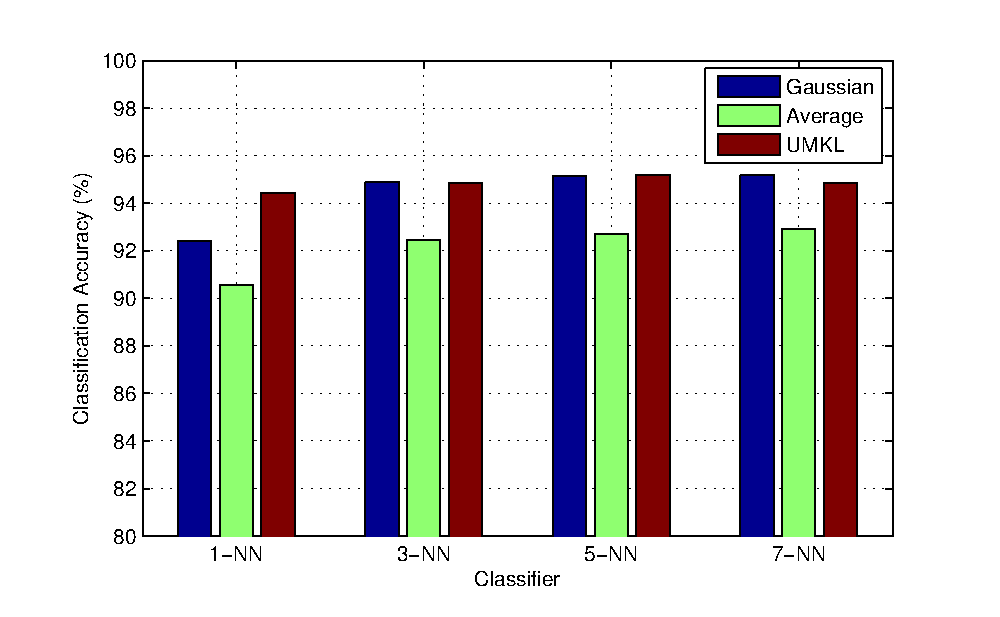
\includegraphics[width=2.5in]{figures/acml-KPCAbreast.eps}
}
\subfigure[Diabetes]{
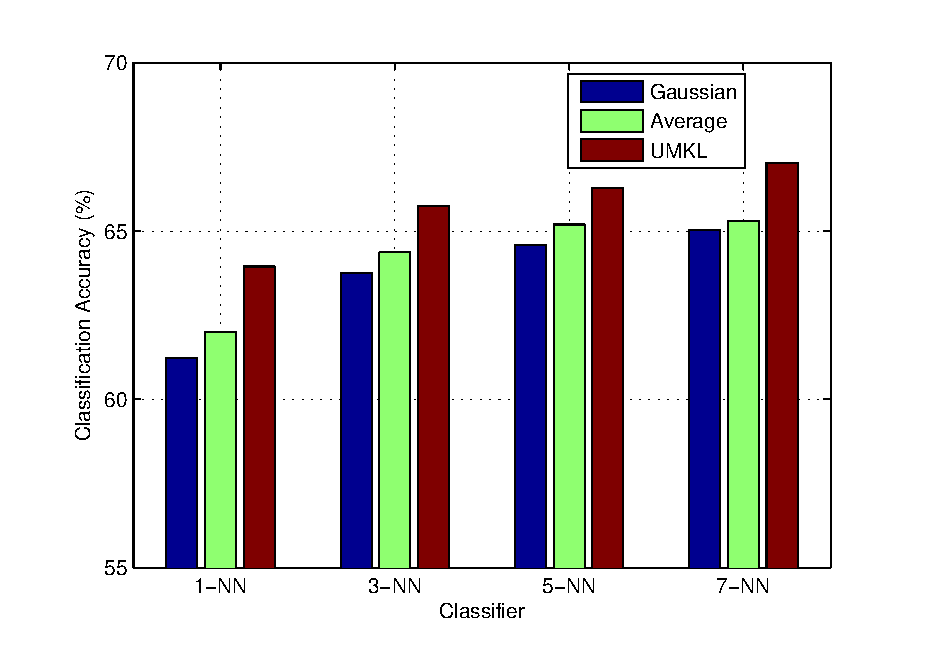
\includegraphics[width=2.5in]{figures/acml-KPCAdiabetes.eps}
}
\subfigure[Flaresolar]{
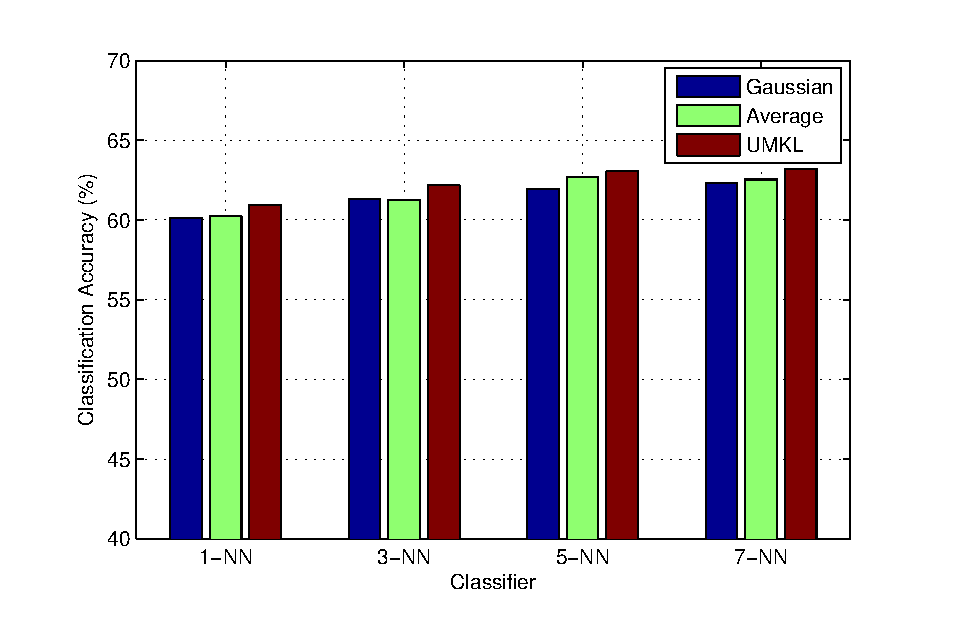
\includegraphics[width=2.5in]{figures/acml-KPCAflaresolar.eps}
}
\subfigure[German]{
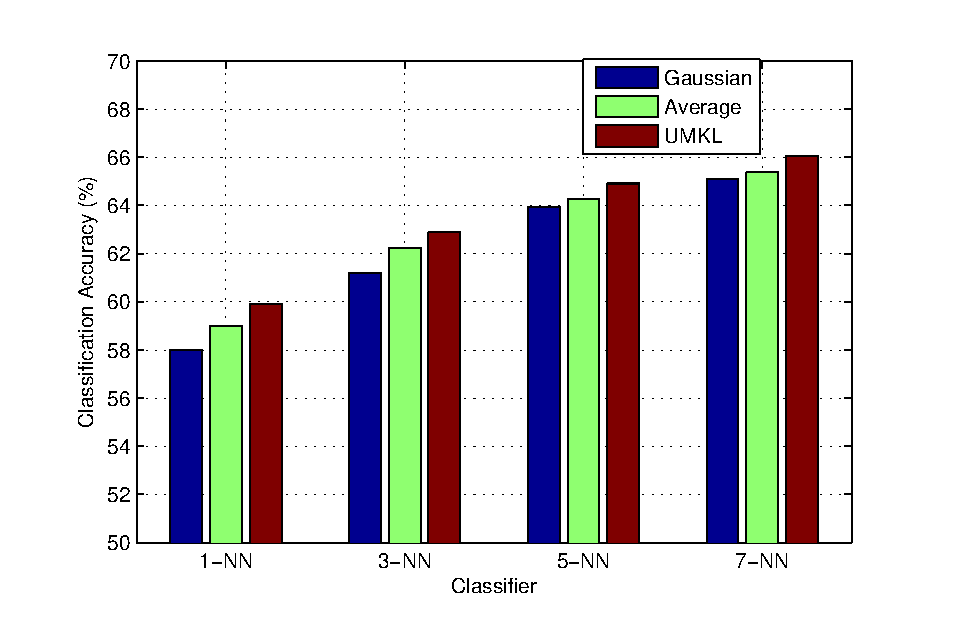
\includegraphics[width=2.5in]{figures/acml-KPCAgerman.eps}
}
\subfigure[Sonar]{
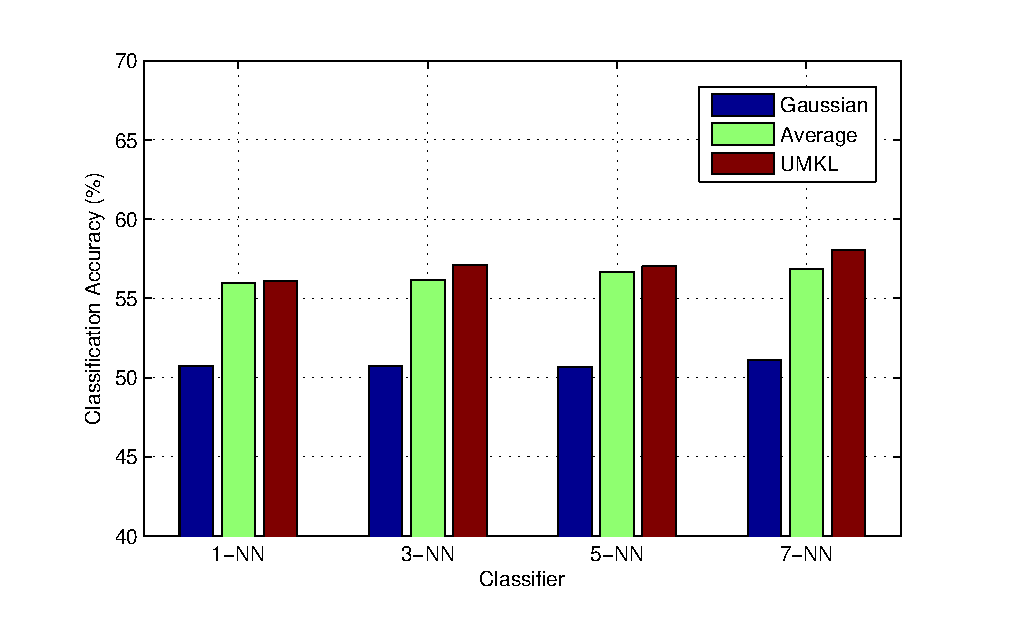
\includegraphics[width=2.5in]{figures/acml-KPCAsonar.eps}
}
\subfigure[Liver]{
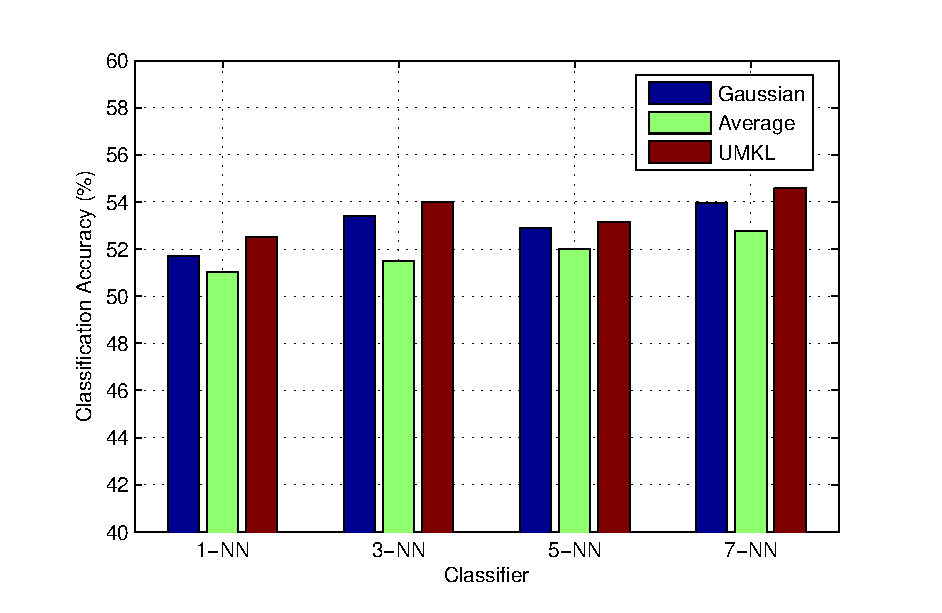
\includegraphics[width=2.5in]{figures/acml-KPCAliver.eps}
}
\caption{The classification accuracy of k-NN after KPCA with Gaussian kernel with sigma=1,the average combination of multiple kernels, the kernel learned by UMKL with varied number of nearest neighbours.}
\end{center}
\end{figure*}

%=======================================================
\section{Summary}\label{sec:acml-con}
%=======================================================

In this chapter we propose a novel unsupervised multiple kernel learning (UMKL) method, which is able to identify an appropriate linear combination of multiple kernels purely from unlabeled data without using class labels. In particular, the proposed UKML approach deems the kernel evaluation result of a data instance as its local coding, and adopts an efficient iterative algorithm to learn the kernel and the local set of basis simultaneously. We apply UKML for two machine learning tasks: (i) kernel learning for choosing appropriate kernels in a classifiction task and (ii) kernel selection in a kernel-based dimension reduction task based on the well-known Kernel PCA technique.  Empirical results show that the classifier using the kernel learned by UMKL is comparable with the state-of-the-art supervised MKL algorithms, and the KPCA scheme using the kernel learned by UKML considerably outperforms the conventional approaches.

